\subsection{Silica gel influence on \ch{O3} and \ch{NO2} concentration}
\label{sec:silica}

\subsubsection{Setup}
\label{sec:silica-setup}

In this experiment we wanted to deduce the influence of the Silica gel
filter, installed behind the Ozone generator, on the \ch{NO2} and
\ch{O3} concentration. For this we used the updated cavity as
described in Section~\ref{sec:inclusion}. This setup was necessary as
the expected \ch{NO2} concentrations were so low, that they were
undetectable by a `longpath' instrument (at the utilized wavelength
range). The disadvantage of this procedure lies in the fact, that the
Ozone absorption in the visible spectrum is much weaker than in the UV
spectrum, such that we have to accept higher uncertainties in the DOAS
fit for this species.

Additionally we did not measure the output of the generator directly,
as the Ozone concentration would have been so high as to damage the cavity's
main stream pump. Therefore we used a setup as depicted
in Figure~\ref{fig:ozone-flow-setup}, which used zero air cartridges at
both the sample air and the zero air input. This allowed us to dilute
the Ozone enriched air by mixing it with the `sample air'. By
utilizing the second zero air cartridge we could guarantee the
measured air to be sufficiently trace gas free and hence kept
additional errors down. 

We took three test series. For all of them the total flow was fixed to
$\Phi = \SI{2}{\liter\per\minute}$ and the Ozone flow $\Phi_{\ch{O3}}$
was varied between \num{0} and \SI{0.3}{\liter\per\minute}. The first
two series were recorded while increasing the Ozone flow, whereas the
last one was measured while decreasing the flow. This was done to
check for any hysteresis effects in the Silica gel. Furthermore for
the second series the Silica gel filter had been removed. For each
flow we waited until the concentrations had stabilized before
averaging over several minutes.

\begin{figure}[htbp]
  \centering
  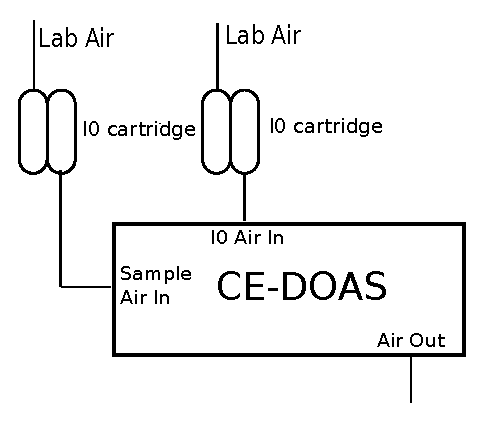
\includegraphics[width=0.35\textwidth]{ozone_setup.eps}
  \caption{Ozone measurement setup.}
  \label{fig:ozone-flow-setup}
\end{figure}

\subsubsection{Results}
\label{sec:silica-results}

The result of our experiment can be found in
Figure~\ref{fig:o3-flow}. The left hand side describes the Ozone
concentration and we can see that hysteresis effects in the Silica gel
are negligible. Within the errors the ascendingly and descendingly
measured Ozone concentration coincide. The Ozone concentration
measured without Silica gel filter differs from the other two, however
differently from what we expected beforehand. The gel should adsorb
some of the Ozone, so it sounds reasonable that the absolute Ozone
concentration \emph{without} filter should be higher than the one
\emph{with} filter. However, as we can see, we measure exactly the
opposite. \todo{why is Ozone level without filter lower?}

Looking at the right hand side of Figure~\ref{fig:o3-flow}, we see the
strong influence of the Silica gel on the \ch{NO2} levels. With
filter, we have no \ch{NO2} signal, without it, we have concentrations
reaching up to \SI{14}{ppb}. This result underlines the stark
improvement of the generator by introducing an additional filtering
stage. We do not have to compensate for additional \ch{NO2} signals,
but can work with Nitrogen Dioxide free generator air. The filter
seems to be a very effective tool to clean the generator air.

\begin{figure}[htbp]
  \centering
  % GNUPLOT: LaTeX picture with Postscript
\begingroup
  \makeatletter
  \providecommand\color[2][]{%
    \GenericError{(gnuplot) \space\space\space\@spaces}{%
      Package color not loaded in conjunction with
      terminal option `colourtext'%
    }{See the gnuplot documentation for explanation.%
    }{Either use 'blacktext' in gnuplot or load the package
      color.sty in LaTeX.}%
    \renewcommand\color[2][]{}%
  }%
  \providecommand\includegraphics[2][]{%
    \GenericError{(gnuplot) \space\space\space\@spaces}{%
      Package graphicx or graphics not loaded%
    }{See the gnuplot documentation for explanation.%
    }{The gnuplot epslatex terminal needs graphicx.sty or graphics.sty.}%
    \renewcommand\includegraphics[2][]{}%
  }%
  \providecommand\rotatebox[2]{#2}%
  \@ifundefined{ifGPcolor}{%
    \newif\ifGPcolor
    \GPcolorfalse
  }{}%
  \@ifundefined{ifGPblacktext}{%
    \newif\ifGPblacktext
    \GPblacktexttrue
  }{}%
  % define a \g@addto@macro without @ in the name:
  \let\gplgaddtomacro\g@addto@macro
  % define empty templates for all commands taking text:
  \gdef\gplbacktext{}%
  \gdef\gplfronttext{}%
  \makeatother
  \ifGPblacktext
    % no textcolor at all
    \def\colorrgb#1{}%
    \def\colorgray#1{}%
  \else
    % gray or color?
    \ifGPcolor
      \def\colorrgb#1{\color[rgb]{#1}}%
      \def\colorgray#1{\color[gray]{#1}}%
      \expandafter\def\csname LTw\endcsname{\color{white}}%
      \expandafter\def\csname LTb\endcsname{\color{black}}%
      \expandafter\def\csname LTa\endcsname{\color{black}}%
      \expandafter\def\csname LT0\endcsname{\color[rgb]{1,0,0}}%
      \expandafter\def\csname LT1\endcsname{\color[rgb]{0,1,0}}%
      \expandafter\def\csname LT2\endcsname{\color[rgb]{0,0,1}}%
      \expandafter\def\csname LT3\endcsname{\color[rgb]{1,0,1}}%
      \expandafter\def\csname LT4\endcsname{\color[rgb]{0,1,1}}%
      \expandafter\def\csname LT5\endcsname{\color[rgb]{1,1,0}}%
      \expandafter\def\csname LT6\endcsname{\color[rgb]{0,0,0}}%
      \expandafter\def\csname LT7\endcsname{\color[rgb]{1,0.3,0}}%
      \expandafter\def\csname LT8\endcsname{\color[rgb]{0.5,0.5,0.5}}%
    \else
      % gray
      \def\colorrgb#1{\color{black}}%
      \def\colorgray#1{\color[gray]{#1}}%
      \expandafter\def\csname LTw\endcsname{\color{white}}%
      \expandafter\def\csname LTb\endcsname{\color{black}}%
      \expandafter\def\csname LTa\endcsname{\color{black}}%
      \expandafter\def\csname LT0\endcsname{\color{black}}%
      \expandafter\def\csname LT1\endcsname{\color{black}}%
      \expandafter\def\csname LT2\endcsname{\color{black}}%
      \expandafter\def\csname LT3\endcsname{\color{black}}%
      \expandafter\def\csname LT4\endcsname{\color{black}}%
      \expandafter\def\csname LT5\endcsname{\color{black}}%
      \expandafter\def\csname LT6\endcsname{\color{black}}%
      \expandafter\def\csname LT7\endcsname{\color{black}}%
      \expandafter\def\csname LT8\endcsname{\color{black}}%
    \fi
  \fi
    \setlength{\unitlength}{0.0500bp}%
    \ifx\gptboxheight\undefined%
      \newlength{\gptboxheight}%
      \newlength{\gptboxwidth}%
      \newsavebox{\gptboxtext}%
    \fi%
    \setlength{\fboxrule}{0.5pt}%
    \setlength{\fboxsep}{1pt}%
\begin{picture}(4030.00,4030.00)%
    \gplgaddtomacro\gplbacktext{%
      \csname LTb\endcsname%
      \put(682,704){\makebox(0,0)[r]{\strut{}$2$}}%
      \put(682,1148){\makebox(0,0)[r]{\strut{}$4$}}%
      \put(682,1592){\makebox(0,0)[r]{\strut{}$6$}}%
      \put(682,2037){\makebox(0,0)[r]{\strut{}$8$}}%
      \put(682,2481){\makebox(0,0)[r]{\strut{}$10$}}%
      \put(682,2925){\makebox(0,0)[r]{\strut{}$12$}}%
      \put(682,3369){\makebox(0,0)[r]{\strut{}$14$}}%
      \put(814,484){\makebox(0,0){\strut{}$0$}}%
      \put(1217,484){\makebox(0,0){\strut{}$0.05$}}%
      \put(1619,484){\makebox(0,0){\strut{}$0.1$}}%
      \put(2022,484){\makebox(0,0){\strut{}$0.15$}}%
      \put(2425,484){\makebox(0,0){\strut{}$0.2$}}%
      \put(2828,484){\makebox(0,0){\strut{}$0.25$}}%
      \put(3230,484){\makebox(0,0){\strut{}$0.3$}}%
      \put(3633,484){\makebox(0,0){\strut{}$0.35$}}%
    }%
    \gplgaddtomacro\gplfronttext{%
      \csname LTb\endcsname%
      \put(176,2036){\rotatebox{-270}{\makebox(0,0){\strut{}Concentration [ppm]}}}%
      \put(2223,154){\makebox(0,0){\strut{}Flow [\si{\liter\per\minute}]}}%
      \put(2223,3699){\makebox(0,0){\strut{}Ozone}}%
    }%
    \gplbacktext
    \put(0,0){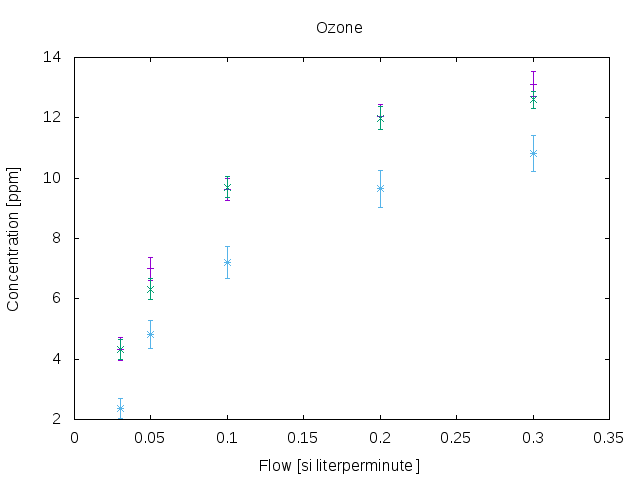
\includegraphics{../images/O3}}%
    \gplfronttext
  \end{picture}%
\endgroup

  \hfill
  % GNUPLOT: LaTeX picture with Postscript
\begingroup
  \makeatletter
  \providecommand\color[2][]{%
    \GenericError{(gnuplot) \space\space\space\@spaces}{%
      Package color not loaded in conjunction with
      terminal option `colourtext'%
    }{See the gnuplot documentation for explanation.%
    }{Either use 'blacktext' in gnuplot or load the package
      color.sty in LaTeX.}%
    \renewcommand\color[2][]{}%
  }%
  \providecommand\includegraphics[2][]{%
    \GenericError{(gnuplot) \space\space\space\@spaces}{%
      Package graphicx or graphics not loaded%
    }{See the gnuplot documentation for explanation.%
    }{The gnuplot epslatex terminal needs graphicx.sty or graphics.sty.}%
    \renewcommand\includegraphics[2][]{}%
  }%
  \providecommand\rotatebox[2]{#2}%
  \@ifundefined{ifGPcolor}{%
    \newif\ifGPcolor
    \GPcolorfalse
  }{}%
  \@ifundefined{ifGPblacktext}{%
    \newif\ifGPblacktext
    \GPblacktexttrue
  }{}%
  % define a \g@addto@macro without @ in the name:
  \let\gplgaddtomacro\g@addto@macro
  % define empty templates for all commands taking text:
  \gdef\gplbacktext{}%
  \gdef\gplfronttext{}%
  \makeatother
  \ifGPblacktext
    % no textcolor at all
    \def\colorrgb#1{}%
    \def\colorgray#1{}%
  \else
    % gray or color?
    \ifGPcolor
      \def\colorrgb#1{\color[rgb]{#1}}%
      \def\colorgray#1{\color[gray]{#1}}%
      \expandafter\def\csname LTw\endcsname{\color{white}}%
      \expandafter\def\csname LTb\endcsname{\color{black}}%
      \expandafter\def\csname LTa\endcsname{\color{black}}%
      \expandafter\def\csname LT0\endcsname{\color[rgb]{1,0,0}}%
      \expandafter\def\csname LT1\endcsname{\color[rgb]{0,1,0}}%
      \expandafter\def\csname LT2\endcsname{\color[rgb]{0,0,1}}%
      \expandafter\def\csname LT3\endcsname{\color[rgb]{1,0,1}}%
      \expandafter\def\csname LT4\endcsname{\color[rgb]{0,1,1}}%
      \expandafter\def\csname LT5\endcsname{\color[rgb]{1,1,0}}%
      \expandafter\def\csname LT6\endcsname{\color[rgb]{0,0,0}}%
      \expandafter\def\csname LT7\endcsname{\color[rgb]{1,0.3,0}}%
      \expandafter\def\csname LT8\endcsname{\color[rgb]{0.5,0.5,0.5}}%
    \else
      % gray
      \def\colorrgb#1{\color{black}}%
      \def\colorgray#1{\color[gray]{#1}}%
      \expandafter\def\csname LTw\endcsname{\color{white}}%
      \expandafter\def\csname LTb\endcsname{\color{black}}%
      \expandafter\def\csname LTa\endcsname{\color{black}}%
      \expandafter\def\csname LT0\endcsname{\color{black}}%
      \expandafter\def\csname LT1\endcsname{\color{black}}%
      \expandafter\def\csname LT2\endcsname{\color{black}}%
      \expandafter\def\csname LT3\endcsname{\color{black}}%
      \expandafter\def\csname LT4\endcsname{\color{black}}%
      \expandafter\def\csname LT5\endcsname{\color{black}}%
      \expandafter\def\csname LT6\endcsname{\color{black}}%
      \expandafter\def\csname LT7\endcsname{\color{black}}%
      \expandafter\def\csname LT8\endcsname{\color{black}}%
    \fi
  \fi
    \setlength{\unitlength}{0.0500bp}%
    \ifx\gptboxheight\undefined%
      \newlength{\gptboxheight}%
      \newlength{\gptboxwidth}%
      \newsavebox{\gptboxtext}%
    \fi%
    \setlength{\fboxrule}{0.5pt}%
    \setlength{\fboxsep}{1pt}%
\begin{picture}(3888.00,3888.00)%
    \gplgaddtomacro\gplbacktext{%
      \csname LTb\endcsname%
      \put(682,862){\makebox(0,0)[r]{\strut{}$0$}}%
      \put(682,1177){\makebox(0,0)[r]{\strut{}$2$}}%
      \put(682,1492){\makebox(0,0)[r]{\strut{}$4$}}%
      \put(682,1808){\makebox(0,0)[r]{\strut{}$6$}}%
      \put(682,2123){\makebox(0,0)[r]{\strut{}$8$}}%
      \put(682,2439){\makebox(0,0)[r]{\strut{}$10$}}%
      \put(682,2754){\makebox(0,0)[r]{\strut{}$12$}}%
      \put(682,3069){\makebox(0,0)[r]{\strut{}$14$}}%
      \put(814,484){\makebox(0,0){\strut{}$0$}}%
      \put(1196,484){\makebox(0,0){\strut{}$0.05$}}%
      \put(1579,484){\makebox(0,0){\strut{}$0.1$}}%
      \put(1961,484){\makebox(0,0){\strut{}$0.15$}}%
      \put(2344,484){\makebox(0,0){\strut{}$0.2$}}%
      \put(2726,484){\makebox(0,0){\strut{}$0.25$}}%
      \put(3109,484){\makebox(0,0){\strut{}$0.3$}}%
      \put(3491,484){\makebox(0,0){\strut{}$0.35$}}%
    }%
    \gplgaddtomacro\gplfronttext{%
      \csname LTb\endcsname%
      \put(176,1965){\rotatebox{-270}{\makebox(0,0){\strut{}Concentration [ppb]}}}%
      \put(2152,154){\makebox(0,0){\strut{}Flow [\si{\liter\per\minute}]}}%
      \put(2152,3557){\makebox(0,0){\strut{}Nitrogen Dioxide}}%
      \csname LTb\endcsname%
      \put(2504,2185){\makebox(0,0)[r]{\strut{}f,  i}}%
      \csname LTb\endcsname%
      \put(2504,1965){\makebox(0,0)[r]{\strut{}f, d}}%
      \csname LTb\endcsname%
      \put(2504,1745){\makebox(0,0)[r]{\strut{}nf, i}}%
    }%
    \gplbacktext
    \put(0,0){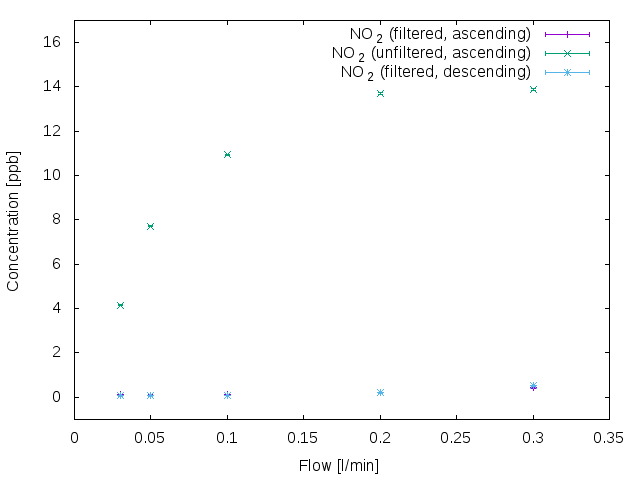
\includegraphics{../images/NO2}}%
    \gplfronttext
  \end{picture}%
\endgroup

  \caption{\ch{O3} and \ch{NO2} concentration over generator flow for
    filtered (f) and not filtered (nf) generator air. And for the two
    cases, where the flow was increased (i) or decreased (d).}
  \label{fig:o3-flow}
\end{figure}

%%% Local Variables:
%%% mode: latex
%%% TeX-master: "../Bachelor"
%%% End:
